\section{群同态：定义、核与像}


参考：[DF] Dummit–Foote《Abstract Algebra》§1.6（定义）、§3.1（Proposition 1）、§3.3（Corollary 17）；[DS]《离散数学与结构》§9.5。

\subsection{定义}


设 $G,H$ 是群。映射 $\varphi:G\to H$ 若对任意 $a,b\in G$ 满足

\[\varphi(ab)=\varphi(a)\varphi(b),\]

称为群同态（homomorphism）。若 $\varphi$ 是单射，称为单同态；若为满射，称为满同态；若既单又满（即双射），称为同构（isomorphism），记 $G\cong H$。

\subsection{同态保持的结构}


设 $e_G,e_H$ 分别是两群的单位元。由

\[\varphi(e_G)=\varphi(e_Ge_G)=\varphi(e_G)^2\]

和消去律得 $\varphi(e_G)=e_H$。又

\[e_H=\varphi(e_G)=\varphi(aa^{-1})=\varphi(a)\varphi(a^{-1}),\]

所以 $\varphi(a^{-1})=\varphi(a)^{-1}$。归纳得 $\varphi(a^n)=\varphi(a)^n$（$n\in\mathbb Z$）。因此若 $|a|$ 有限，则 $|\varphi(a)|$ 整除 $|a|$；同构保持元素的阶。

\subsection{核与像}


\[ \operatorname{im}\varphi=\varphi(G)=\{\varphi(g):g\in G\}\le H,\qquad \ker\varphi=\{g\in G:\varphi(g)=e_H\}\le G. \]

像（image）是目标群中被映到的部分，核（kernel）是被映到单位元的元素。

验证 $\ker\varphi\le G$：对 $g,g'\in\ker\varphi$，

\[\varphi\bigl(g\,(g')^{-1}\bigr)=\varphi(g)\,\varphi(g')^{-1}=e_He_H^{-1}=e_H,\]

由子群判定准则即得。

核是正规子群：若 $k\in\ker\varphi$，$g\in G$，则

\[\varphi(gkg^{-1})=\varphi(g)\,e_H\,\varphi(g)^{-1}=e_H,\]

所以 $gkg^{-1}\in\ker\varphi$，即 $\ker\varphi\trianglelefteq G$。

\subsection{单射与满射}


同态满足

\[\varphi\ \text{单射}\iff\ker\varphi=\{e_G\}.\]

证明：若 $\varphi(a)=\varphi(b)$，则

\[\varphi(ab^{-1})=\varphi(a)\varphi(b)^{-1}=e_H,\]

即 $ab^{-1}\in\ker\varphi$；核平凡时 $a=b$。反之若 $k\in\ker\varphi$，则 $\varphi(k)=\varphi(e_G)$，单射给出 $k=e_G$。满射等价于 $\operatorname{im}\varphi=H$。

\subsection{例}


1. 行列式 $\det:GL_n(F)\to F^\times$ 是满同态，核为
\[\operatorname{SL}_n(F)=\{A\in GL_n(F):\det A=1\}.\]
对任意 $c\in F^\times$，矩阵 $\operatorname{diag}(c,1,\ldots,1)$ 的行列式是 $c$，所以满射。

2. 对 $N\trianglelefteq G$，映射 $\pi:G\to G/N$，$\pi(g)=gN$，是满同态且 $\ker\pi=N$。

\subsection{同态的纤维}


对 $h\in\operatorname{im}\varphi$，纤维（fiber）$\varphi^{-1}(h)$ 是核的一个陪集：

\[\varphi^{-1}(h)=g\ker\varphi\qquad(\text{任取 } g \text{ 使 } \varphi(g)=h).\]

因为 $x\in\varphi^{-1}(h)\iff\varphi(g^{-1}x)=e_H\iff g^{-1}x\in\ker\varphi$。于是同态把定义域按核的陪集分块，这正是第一同构定理的直观。


\begin{center}
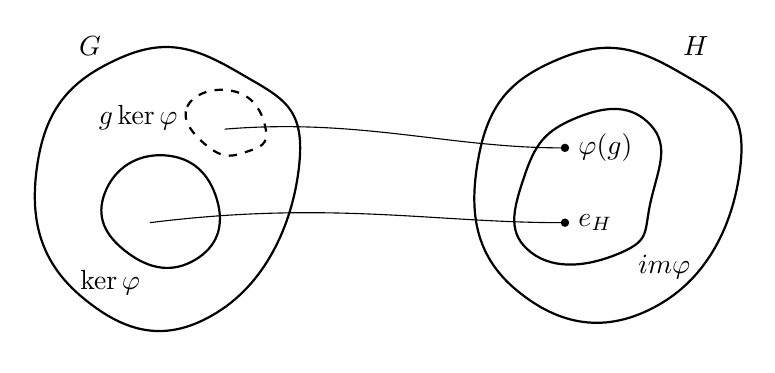
\begin{tikzpicture}[scale=0.95]
  \draw[thick] plot[smooth cycle, tension=0.85] coordinates {(-2.9,-1.5) (-3.5,0.3) (-2.4,1.7) (-0.8,1.5) (0.0,0.3) (-1.1,-1.7)};
  \draw[thick] plot[smooth cycle, tension=0.85] coordinates {(2.9,-1.4) (2.4,0.4) (3.5,1.7) (5.1,1.5) (5.9,0.3) (4.8,-1.6)};
  \node[above] at (-2.8,1.6) {$G$};
  \node[above] at (5.3,1.6) {$H$};
  \draw[thick] plot[smooth cycle, tension=0.9] coordinates {(-2.3,-0.9) (-2.6,-0.1) (-1.8,0.4) (-1.1,-0.2) (-1.4,-1.0)};
  \node[below left] at (-2.0,-1.0) {$\ker\varphi$};
  \draw[thick,dashed] plot[smooth cycle, tension=0.9] coordinates {(-1.2,0.5) (-1.5,1.05) (-0.85,1.25) (-0.45,0.75) (-0.7,0.45)};
  \node[left] at (-1.5,0.9) {$g\ker\varphi$};
  \draw (-2.0,-0.5) .. controls (0.4,-0.2) and (1.8,-0.5) .. (3.5,-0.5);
  \fill (3.55,-0.5) circle (1.6pt);
  \node[right] at (3.6,-0.5) {$e_H$};
  \draw (-1.0,0.75) .. controls (0.8,0.9) and (2.0,0.5) .. (3.5,0.5);
  \fill (3.55,0.5) circle (1.6pt);
  \node[right] at (3.6,0.5) {$\varphi(g)$};
  \draw[thick] plot[smooth cycle, tension=0.9] coordinates {(3.1,-0.9) (3.0,0.1) (3.7,0.9) (4.7,0.8) (4.7,-0.2) (4.3,-0.9)};
  \node[below right] at (4.4,-0.8) {$\operatorname{im}\varphi$};
\end{tikzpicture}
\\[4pt]
{\small 图：同态把每个陪集（纤维）压成一点：$\ker\varphi$ 压到 $e_H$，陪集 $g\ker\varphi$ 压到 $\varphi(g)$。}
\end{center}
